\section{System dialogów (Bartosz Strzelecki)}

W naszej implementacji konwersacje składają się z dwóch rodzajów węzłów. Jednego odpowiedzialnego za wypowiedzi postaci niezależnych oraz drugiego
pozwalającego na podjęcie przez gracza decyzji.
Dodanie nowej konwersacji odbywa się poprzez stworzenie obiektu z przypisanym komponentem NPC Conversation.
Wywołanie dialogu można osiągnąć poprzez wykorzystanie metody


\begin{verbatim}
ConversationManager.Instance.StartConversation(/*NPCConversation*/);
\end{verbatim}

\begin{figure}[h]
\centering
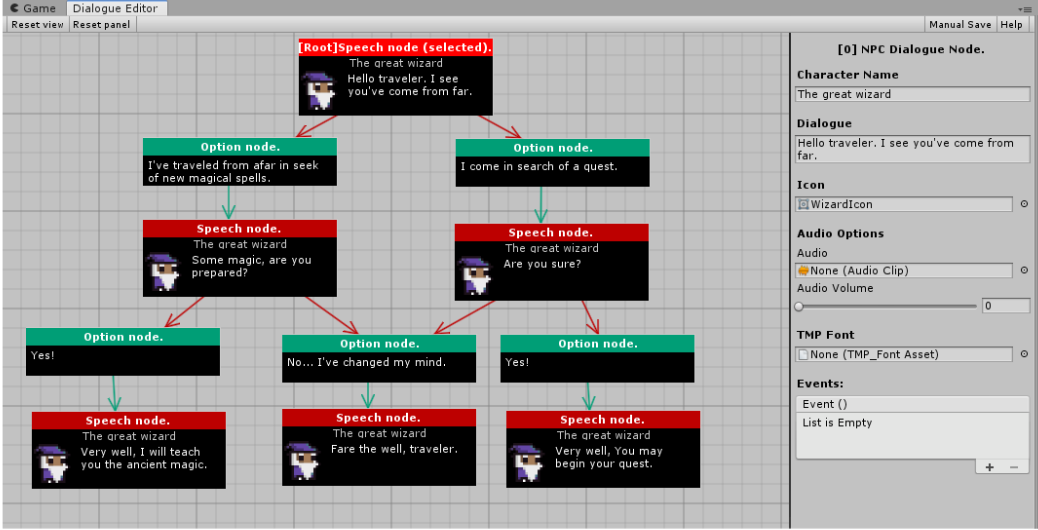
\includegraphics[width=0.6\textwidth]{images/dial}
\caption{Przykładowa konwersacja z wykorzystaniem Dialogue Editor}
\end{figure}
System pozwała na łatwe dostosowanie elementów interfejsu użytkownika odpowiedzialne za wyświetlenie dialogów, aby jak najlepiej wpasować się
w styl graficzny gry.

\begin{figure}[h]
\centering
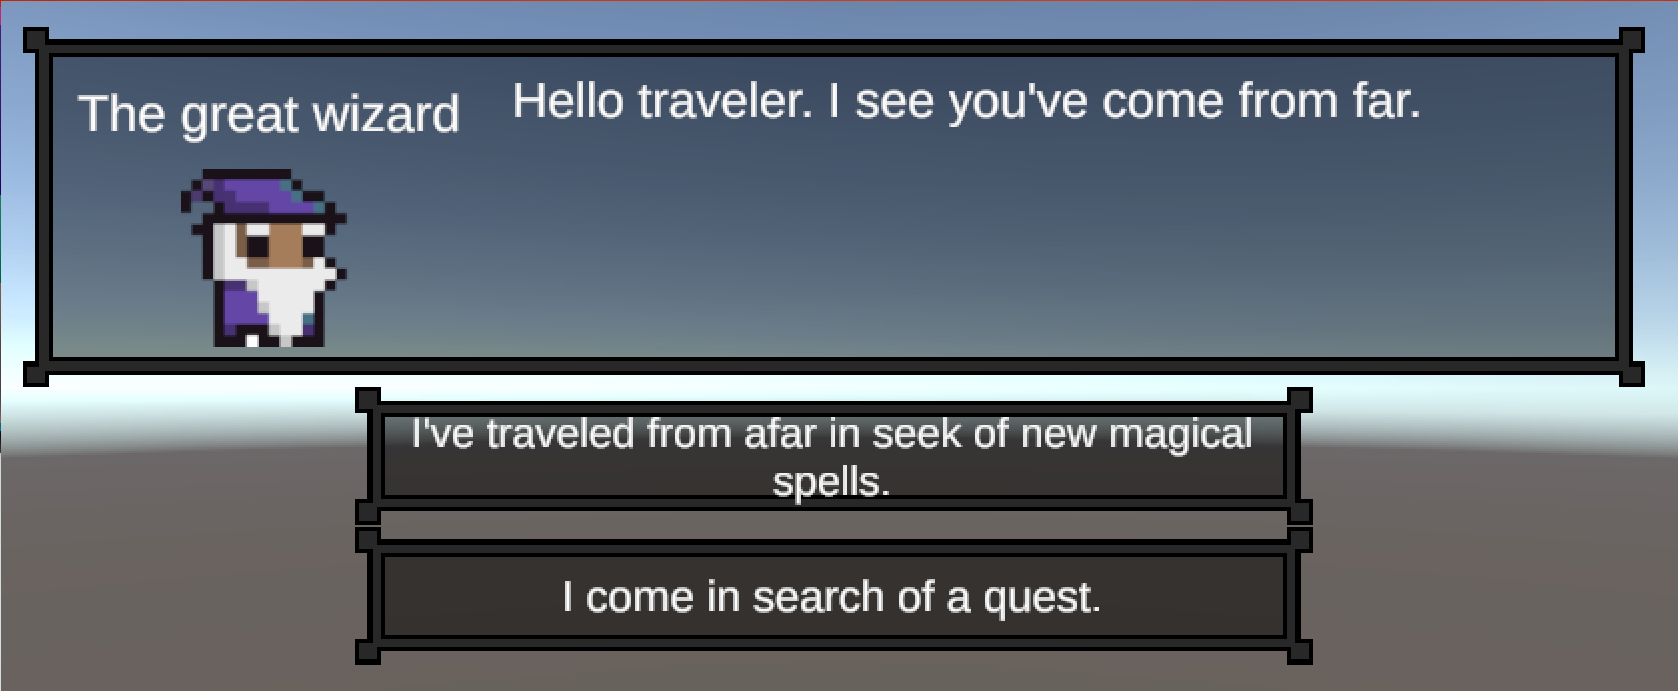
\includegraphics[width=0.6\textwidth]{images/d}
\caption{Przykładowe okno dialogowe widziane z perspektywy gracza.}
\end{figure}
